\documentclass[12pt]{report}
\usepackage{geometry}
\geometry{hmargin=2cm,vmargin=1.5cm}

\usepackage{hyperref}
\usepackage[T1]{fontenc}
\usepackage[utf8]{inputenc}
\usepackage[francais]{babel}

\usepackage{graphicx}

\title{Rapport de stage \\
Licence Informatique 3\up{ème} année}
\author{stagiaire : Athman Mekhzoumi\\
tuteur : Olivier Baudon} 

\begin{document}
\newpage
\maketitle
\tableofcontents
\newpage

\chapter{Introduction au stage}

Dans cette partie, je vais présenter le thème du stage, les prérequis exigés, le travail demandé et dans quel contexte ce sujet a été posé.

\section{Sujet du stage}

Le sujet du stage est \textit{Publier une bibliothèque sur les graphes et la compléter}, une version non complète de la bibliothèque était déjà implémentée avant le début du stage, les tâches principales étaient de compléter le code là où il y manquait, améliorer le code en s'inspirant des nouvelles versions du langage \textit{Java} et aussi commenter la bibliothèque.\newline

Des connaissances en "programmation orienté objet" et en "Théorie des graphes" m'était nécessaire pour comprendre la conception et l'implémentation de la bibliothèque, heureusement pour moi j'avais déjà acquis les notions de base sur ces deux domaines au cours de mes études universitaires dans mon pays natal, mais cela ne m'était pas suffisant car il me fallait des connaissances plus profondes, alors j'ai lu quelques cours en ligne et coder des petits programmes avant le début du stage pour être au niveau exigé. 

\section{Le contexte du stage}

Ce stage rentre dans le cadre du cycle licence, c'est un stage obligatoire de 4 semaines minimum, il représente l'élément pédagogique 4 TTVP18U et il fait partie du semestre 6 du parcours informatique, l'obtention de ce stage était fait avec une candidature spontanée adressée à l'enseignant-chercheur du labri Mr BAUDON Olivier.

\newpage
\chapter{Déroulement du stage}

Dans cette partie je vais présenter mon travail, les compétences que j'ai mobilisées pour le réaliser ainsi que les connaissances et compétences acquises et maîtrisées.

\section{première semaine}

\subsection{Les classes abstraites et les interfaces}

Une classe est définie comme abstraite avec le mot-clé \textbf{abstract}, les classes abstraites sont à utiliser lorsqu'une classe mère ne doit pas être instanciée, cette dernière peut t'avoir ce qu'on appelle une méthode abstraite qui est caractérisée par le fait qu'elle n'a pas de corps, comme elle peut t'avoir des méthodes normales, par contre si une classe contient une méthode abstraite, cette classe doit alors être déclarée abstraite.\newline

Une interface n'est qu'une classe abstraite à 100\%, ce qui signifie aucune méthode d'une interface n'a de corps, elle sert à définir un super-type et à utiliser le polymorphisme, pour implémenter dans une classe il faut utiliser les mots-clés \textbf{implements}, et on peut implémenter autant qu'on veut dans la même classe, pour que cela soit fait correctement il faut redéfinir toutes les méthodes de l'interface (ou des interfaces) dans la classe concernée.

\subsection{Les exceptions}
Lorsqu'un événement que la JVM ne sait pas gérer apparaît, une exception est levée (exemple : division par zéro). une exception correspond donc à une erreur, la superclasse qui gère les exceptions s'appelle \textbf{Exception}. C'est possible aussi de créer une classe d'exception personnalisée qui génère ce que le programmeur considère comme exception mais peut n'être pas par le JVM, pour y procéder il faut lui hériter de la classe exception.\newline

L'instruction qui permet de capturer des exceptions est le bloc \textbf{Try{…}catch{}}, si une exception est levée dans le bloc Try, les instructions figurant dans le bloc catch seront exécutées pour autant que celui-ci capture la bonne exception levée. On peut aussi prévenir la JVM qu'une méthode est risque de générer une exception grâce au mot-clé \textbf{throws}. Une instanciation d'une exception est lancée par le biais de l'instruction \textbf{throw}.
\newpage

~\\
\subsection{Les varargs}
Les varargs permettent de passer un nombre variable d’arguments à une méthode (pourvu qu’ils soient tous du type déclaré dans la signature de la méthode), sans créer explicitement de tableau, en revanche, dans le corps de la méthode, la variable var-arg est considéré comme un banal tableau et peut donc être parcourue par un « foreach », fournir sa taille avec la propriété length.\newline

Il y a toutefois deux petites limitations à cette syntaxe :

\begin{itemize} 
\item Il ne peut y avoir qu’un seul var-arg par signature de méthode.
\item le var-arg doit toujours être le dernier paramètre.
\end{itemize}

~\\
\section{Deuxième semaine}

\subsection{Les collection}
Les collections permettent de stocker un nombre variable d'objets, il y a principalement trois types de collection : \textbf{Liste} et \textbf{Set} qui hérite de l'interface Collection et aussi le type \textbf{Map}. chaque type a ses avantages et ses inconvénients et fournit des fonctionnalités propres à lui.\newline

Voici quelques différences les différents types de collections;
\begin{itemize}
\item les Collection stockent des objets alors que les Map stockent un couple (clé-valeur).
\item Si on insère fréquemment des données en milieu de liste, \textbf{LinkedList} est plus approprié.
\item si on veut rechercher ou accéder à une valeur via une clé de recherche, vaut mieux opter pour une collection du type \textbf{Map}.
\item si on veut traiter une grande quantité de données, le type \textbf{Set} convient le plus.
\end{itemize}

\subsection{La généricité}
La généricité est un concept très utile pour développer des objets travaillant avec plusieurs types de données, ça nous fait gagner du temps au lieu de développer des classes qui traitent de façon identique des données du types différents.\newline

On peut utiliser la généricité sur les objets servant à gérer des collections, et avec l'outil \textbf{wildcard (?)} ont indiqué que n'importe quel type peut être traité, mais cela revient à rendre ladite collection en lecture seule ce qui peut-être désavantage. 

\newpage
\subsection{Git}
Pour Faciliter la communication et entre le stagiaire et l'encadrant pendant tout le stage, même les weekends, la plate-forme github a été utilisée par pour sauvegarder les changements fait sur la bibliothèque et aussi pour encadrer et guider le stagiaire aux furies et à mesure de son apprentissage.

~\\
\section{Troisième semaine}

\subsection{Diagramme UML}

La modélisation UML permet de vulgariser les aspects liés à la conception et à l’architecture, propres au logiciel (dans ce cas la bibliothèque), au client (dans ce cas les utilisateurs de cette dernière). Aussi, elle apporte une compréhension rapide du programme à d’autres développeurs externes en cas de reprise du logiciel et facilite sa maintenance. \newline

Pour ce projet j'ai utilisé \textbf{ObjectAid UML Explorer} qui est un outil de visualisation de code souple et léger pour l'IDE Eclipse. Il affiche le code source Java et les bibliothèques dans des diagrammes de classes et de séquences UML dynamiques qui se mettent automatiquement à jour lorsque mon code change.\newline

La figure suivante représente les diagrammes UML obtenus à partir d'ObjectAid et en précisant les paramètres souhaités ;
\newpage

\begin{center}
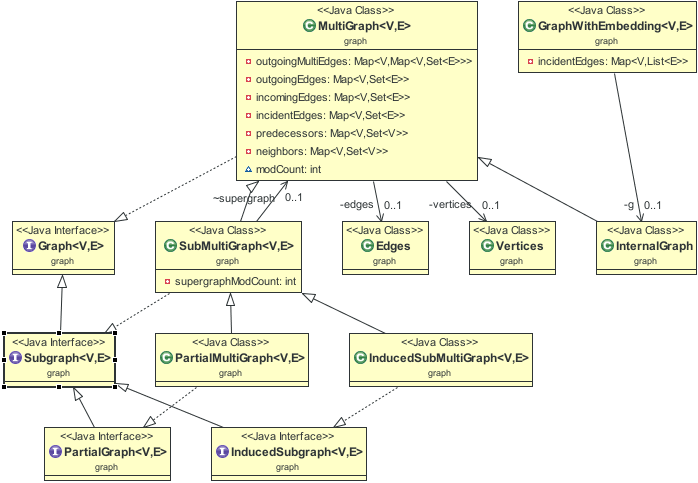
\includegraphics[width=1\textwidth]{DiagUMLPartie1.png}
\caption{\label{fig:DiagUMLPartie1}}
~\\
~\\
~\\
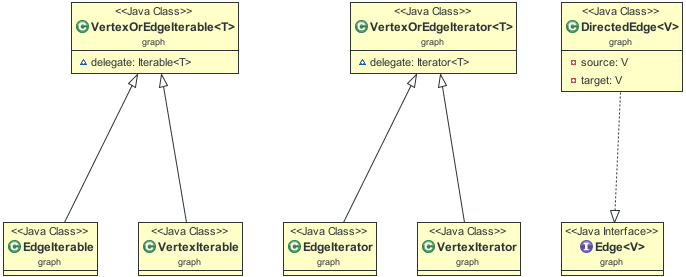
\includegraphics[width=1\textwidth]{DiagUMLPartie2.png}
\caption{\label{fig:DiagUMLPartie2}\newline Figure 1: \textit{Diagrammes UML du package "graphe" }}
\end{center}

\newpage
~\\
\subsection{Classe interne, locale et anonyme}

Une classe interne est déclarée à l'intérieur d'une autre classe, Elle peut donc accéder aux membres de la classe externe. Il yas deux models principales de cette dernière, les classes internes statiques qui ne peuvent accéder qu'aux membres statiques de leurs classes englobantes respectives, les classes internes non statiques qui peuvent accéder aux membres statiques de leurs classes ainsi qu'aux membres des objets respectives qui les ont créées.\newline

Une classe interne définie dans un bloc est une classe interne dont la portée est limitée au bloc : c’est une classe interne locale. Une classe locale ne peut pas être static. Une classe locale peut accéder aux attributs de la classe englobante ainsi qu'aux paramètres et variable locales de la méthode où elle est définie, à condition que ceux-ci soient spécifiés finals.\newline 

Il est possible de définir une classe interne, sans lui donner de nom par dérivation d'une super classe, ou par implémentation d’une interface, c'est ce qu'on appelle une classe anonyme. Elles ont utile lorsqu'on a besoin de déclarer une classe pour l'utiliser une seule fois.\newline


\subsection{Corretion des warnings}

Au début du stage la bibliothèque contenait multiples warning, pour toutes sortes de dysfonctionnement ou de problème éventuelle il fait retirer ces warnings. Pour cela chaque warning a été traité individuellement selon le problème qui le génère. Pour procéder à cette opération j'ai eu recours à deux solutions : les solutions proposées sur internet et l'utilitaire de réparation des warnings intégré a l'IDE Ecplise.
~\\

\section{Quatrième semaine}

\subsection{Optimisation du code}

Une des éthiques de la programmation est la lisibilité du code, donc j'ai essayé de donner à la bibliothèque un code un peu plus lisible et facile à faire. \newline

J'ai donné à quelque interface un nom plus court, par exemple j'ai ajouté \textit{import static graphe. Graph. Edge;} pour avoir \textit{Edge} au lieu de \textit{Graph. Edge}.\newline

Pour améliorer la taille du code et ça visitait, j'ai eu recours à la nouveauté de java 8 \textbf{les expressions lambda}.

\newpage
~\\
\subsection{Lambda expression}

Les expressions lambda sont parmi les nouveaux concepts introduits dans Java 8, leur intérêt est la redéfinition d'une méthode d'une interface fonctionnelle sans avoir à faire une classe anonyme, donc gain de ligne de code et de visibilité.\newline

le sytaxe des lambdas expressions est le suivant :\newline
\textit{(param1, param2, ...) -> \{traitements ; retourne une valeur;\} ;} \newline

Je les ai utilisé dans plusieurs classes de pckage différents, surtout dans la classe \textit{iterables} du package \textit{collections} et la classe \textit{RootedSpanningTreelmpl} du package \textit{util}.\newline

\subsection{Entête et licence}

Pour publier un programme (publiothèque, application, logiciel, ....) développer par soi-même ou en collaboration avec une équipe, il est très important de lui attribuer les copyrights désirer et la licence adéquate, cela permet de protéger le programme et définit avec son cocontractant (exploitant ou utilisateur) les conditions dans lesquelles ce programme peut être utilisé, diffusé ou modifié.\newline

J'ai utilisé le plugiciel d'éclipse \textbf{Éclipse copyright Generator}, pour appliquer un commentaire d'en-tête de copyright à tous les fichiers sources dans les projets, ainsi pour ajouter une licence GNU \textbf{Lesser Général Public Licence v3.0} souhaiter par le tuteur de stage.\newline 

voici une copie de l'en-tête de copyright utiliser dans le projet:\newline

\begin{center}
\textit{Copyright (C) 2018 Olivier Baudon}

\textit{This program is free software: you can redistribute it and/or modify}
\textit{it under the terms of the GNU Lesser General Public License as published by}
\textit{the Free Software Foundation, either version 3 of the License, or}
\textit{(at your option) any later version.}

\textit{This program is distributed in the hope that it will be useful,}
\textit{but WITHOUT ANY WARRANTY; without even the implied warranty of}
\textit{MERCHANTABILITY or FITNESS FOR A PARTICULAR PURPOSE.  See the}
\textit{GNU Lesser General Public License for more details.}

\textit{You should have received a copy of the GNU Lesser General Public License}
\textit{along with this program.  If not, see <http://www.gnu.org/licenses/>.}
\end{center}

\chapter{Bilan du stage} 

\section{Bilan}

Le stage était réparti en deux parties, une première partie théorique et la deuxième pratique.\newline

La partie théorique été très importante pour moi, elle permet de construire base solide en Java et d'enrocher mes connaissances en théorie des graphes. En premier temps j'ai consacré mon temps à comprendre en détaillent les piliers de ce langage, que je connaissais avant, mais je ne le m'égrisais pas bien. comprendre et maîtriser les exceptions et la généricité est un grand plus à mes connaissances d'informaticien, je les ai trouvés très utiles, et rendais le code plus souple et robuste.\newline

La partie pratique m'a permis de mettre en oeuvre ce que j'ai aprit précédemment, j'ai rencontré quelques difficultés à trouver la bonne syntaxe pour quelques cas, mais ça n'a pas duré avec l'aide du tuteur et de l'internet, une fois que j'ai les lambdas expressions, je les ai trouvés très utilisé et facile de mettre en oeuvre. \newline

Ce stage est un grand plus moi, en premier lieu j'ai apris à comprendre un code déjà écrit et savoir le modifier/améliorer sans affecter les autres parties du programme, ainsi que mériter beaucoup mieux la programmation orientée objet, en utilisant le langage Java. J'ai apris aussi à utiliser les plugins pour accélérer le rythme du travaille, tel que les outiles pour tracer des diagrammes UML ou pour génér copyright/licences.

\newpage
\section{Référence}
\begin{verbatim}
https://openclassrooms.com/courses/apprenez-a-programmer-en-java/
les-classes-abstraites-et-les-interfaces

https://openclassrooms.com/courses/apprenez-a-programmer-en-java/
les-exceptions

http://thecodersbreakfast.net/index.php?post/2008/07/23/77-java-les-var-args

https://openclassrooms.com/courses/apprenez-a-programmer-en-java/
les-collections-d-objets

http://objectaid.com/

http://imss-www.upmf-grenoble.fr/prevert/Prog/Java/CoursJava/classes3.html

https://openclassrooms.com/courses/apprenez-a-programmer-en-java/classes-anonymes-interfaces-fonctionnelles-lambdas-et-references-de-methode

https://jmini.github.io/Eclipse-Copyright-Generator/

https://fr.wikipedia.org/wiki/Licence_de_logiciel
\end{verbatim}

\end{document}
